\chapter{Evaluation}
Kleine eingebettete Systeme weisen eine stark limitierte Hardware auf. Dafür sind sie aber sehr klein und verbrauchen wenig Energie. Verschiedene Konfigurationen wurden in dieser Arbeit untersucht. Die gefundene
Lösung muss nicht nur eine hohe Klassifizierungsgenauigkeit erzielen, sondern auch lauffähig auf einem kleinen eingebetteten System sein, d. h. nicht mehr als den verfügbaren RAM und Programmspeicher nutzen und in
einer akzeptablen Zeit terminieren.
\newline
\newline
Dieses Kapitel untersucht zuerst die Klassifizierungsgenauigkeit der besten Konfigurationen, die gefunden wurden, je Feature-Menge. Die beste Konfiguration wird anschließend auf die Ausführungszeit
und Ressourcenverbrauch auf dem ATmega328P hin analysiert. Dabei wird auf mögliche Optimierungen eingegangen, um die Ausführungszeit und den Ressourcenverbrauch zu senken.

\section{Klassifizierungsgenauigkeit}
Es werden drei Features näher betrachtet. Motion History, Helligkeitsverteilung und Schwerpunktverteilung. Daraus wurden vier Feature-Mengen generiert, die zum Trainieren genutzt werden. Insgesamt wurden 22528
verschiedene Konfigurationen trainiert und getestet, die in Kapitel \ref{sec:Training} beschrieben wurden. Jede Konfiguration nutzt zum Trainieren eine Kombination aus der Trainingsmenge von Feng und Kubik,
sowie die Gestentestmenge und die Nullgestenmenge, die in Kapitel \ref{sec:DymelData} beschrieben wurden. Die Trainingsmenge beinhaltet insgesamt 7629 Handgesten. Davon wird 50\% zum Trainieren und 50\% zum
Validieren und Optimieren auf Basis der Monte Carlo Methode benutzt.
\newline
\newline
Unter jeder Feature-Menge werden jeweils drei Kategorien analysiert. Die erste Kategorie zeigt die beste Konfiguration, die ohne Restriktion des Programmspeichers gefunden wurde. Die zweite Kategorie hat eine Restriktion
von 48 kB und die dritte Kategorie hat eine Restriktion von 32 kB. Diese beziehen sich auf den Programmspeicher des ATmega4809 und ATmega328P, die im Rahmen der Fallstudie verwendet werden \cite{venzkeArticle}.
Dabei werden immer 4 kB abgezogen, da diese für andere systemrelevante Funktionen reserviert sind. Die beste Konfiguration einer Kategorie maximiert die Summe
der Klassifizierungsgenauigkeiten der Testmenge von Klisch, der Gestentestmenge und der Nullgestentestmenge. Dabei wird stets die optimierte Programmgröße der Konfiguration betrachtet, nachdem alle Optimierungen aus Kapitel
\ref{sec:eval_size} angewendet wurden.
\newline
\newline
In der Analyse werden die verschiedenen Feature-Mengen im Hinblick auf die Klassifizierungsgenauigkeit der Testmenge von Klisch, der Gestentestmenge, der Nullgestentestmenge und den synthetischen
Helligkeitstestmengen untereinander verglichen und mit den Ergebnissen von Giese verglichen. Es wird ausschließlich mit Giese verglichen, da seine Ergebnisse die beste Klassifizierungsgenauigkeit,
geringste Ausführungszeit und geringsten Ressourcenverbrauch erzielte. Außerdem wird die Auswirkung von verschiedenen Waldgrößen auf die Klassifizierungsgenauigkeit untersucht. Anzumerken ist, dass
lediglich die Testmenge von Klisch vergleichbar mit den Ergebnissen von Giese ist, da die Gestentestmenge, Nullgestentestmenge und Helligkeitstestmengen erst im Laufe dieser Arbeit entstanden sind.

\subsection{Helligkeitsverteilung}
\begin{table}[h!]
    \centering
    \begin{tabular}{ | l | c | c | c |}
        \hline
        Konfiguration & Beste & Unter 44 kB & Unter 28 kB \\\hline
        Ensemble-Methode & ExtraTrees & ExtraTrees & ExtraTrees \\\hline
        Maximalhöhe & 14 & 10 & 15 \\\hline
        Waldgröße & 10 & 6 & 1 \\\hline
        Blattgröße (min\_samples\_leaf) & 4 & 4 & 4 \\\hline
        Programmgröße in Bytes & 76628 & 33284 & 9364 \\\hline
        Genauigkeit Testmenge von Klisch & 74,0\% & 63,5\% & 67,7\% \\\hline
        Genauigkeit Gestentestmenge & 74,1\% & 79,2\% & 76,6\% \\\hline
        Genauigkeit Nullgestentestmenge & 69,0\% & 71,0\% & 67,0\% \\\hline
    \end{tabular}
    \caption{Die beste Konfigurationen der Helligkeitsverteilung.}
    \label{tab:helligkeitsverteilung}
\end{table}
\begin{figure}[h!]
    \centering
    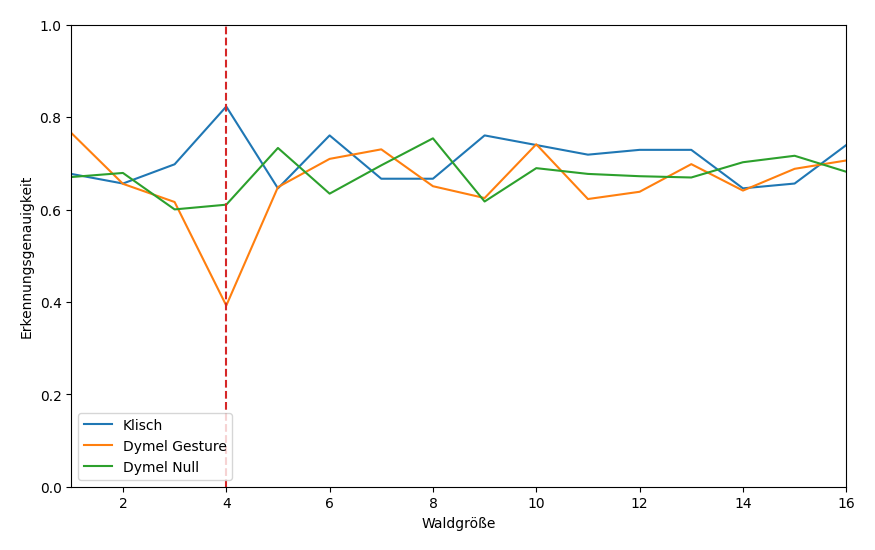
\includegraphics[width=\linewidth]{images/helligkeitsverteilung_acc_per_size.png}
    \caption{Die besten Konfigurationen pro Waldgröße mit der Helligkeitsverteilung.}
    \label{fig:helligkeitsverteilung_per_forest_size}
\end{figure}
Die Featuremenge der Helligkeitsverteilung beinhaltet insgesamt 12 Features. Jeweils 6 Feature repräsentieren Zeitfenster der minimalen Helligkeit und der maximalen Helligkeit. Die Zeitfenster wurden
geometrisch zusammengefasst.
\newline
\newline
Aus der Tabelle \ref{tab:helligkeitsverteilung} sind die besten Konfigurationen jeder Kategorie zu entnehmen. Die beste Konfiguration wurde mit der Ensemble-Methode \textit{ExtraTrees} gefunden.
Sie erzielt eine Klassifizierungsgenauigkeit von 74\% auf der Testmenge von Klisch und ist damit 25,2\% schlechter als das neuronale Netzwerk von Giese \cite{gieseThesis}. Außerdem wird 74\% der Gestentestmenge
und 69\% der Nullgestentestmenge korrekt klassifiziert.
\newline
\newline
Wird die Kategorie \textit{Beste} und die Kategorie \textit{Unter 28 kB} vergleichen, nimmt die Gesamtklassifizierungsgenauigkeit nur um 1,94\% ab. Dabei reduziert sich die Programmgröße um 87,8\%.
Ein ähnliches Verhalten ist auch in Abbildung \ref{fig:helligkeitsverteilung_per_forest_size} zu erkennen. Dort ist nur ein geringer Zuwachs der Gesamtklassifizierungsgenauigkeit mit der zunehmenden
Waldgröße zu beobachten.
\subsection{Motion History}
\begin{table}[h!]
    \centering
    \begin{tabular}{ | l | c | c | c |}
        \hline
        Konfiguration & Beste & Unter 44 kB & Unter 28 kB \\\hline
        Ensemble-Methode & ExtraTrees & ExtraTrees & ExtraTrees \\\hline
        Maximalhöhe & 10 & 11 & 9 \\\hline
        Waldgröße & 16 & 7 & 6 \\\hline
        Blattgröße (min\_samples\_leaf) & 1 & 2 & 1 \\\hline
        Programmgröße in Bytes & 84200 & 40456 & 22804 \\\hline
        Genauigkeit Testmenge von Klisch & 68,8\% & 67,7\% & 62,5\% \\\hline
        Genauigkeit Gestentestmenge & 74,5\% & 67,6\% & 68,5\% \\\hline
        Genauigkeit Nullgestentestmenge & 68,3\% & 64,4\% & 67,6\% \\\hline
    \end{tabular}
    \caption{Die besten Konfigurationen der Feature-Menge Motion History.}
    \label{tab:motion_history}
\end{table}
\begin{figure}[h!]
    \centering
    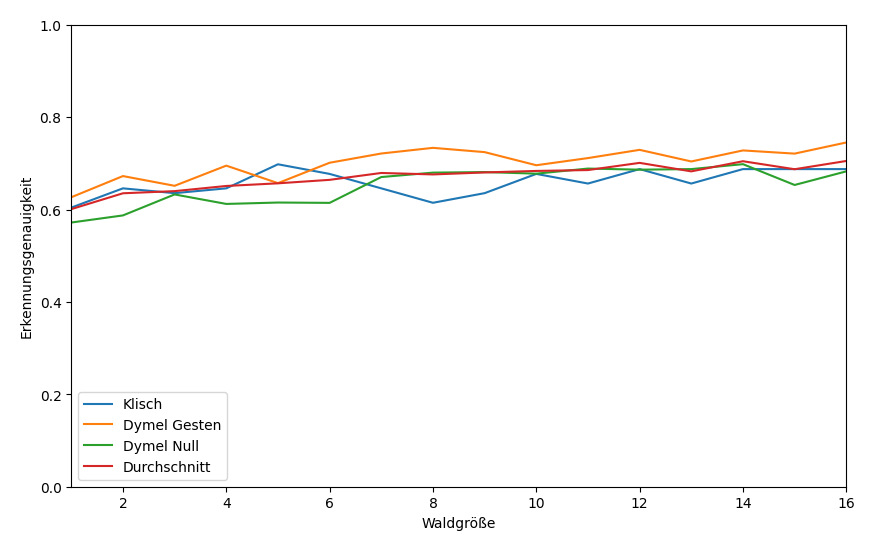
\includegraphics[width=\linewidth]{images/motion_history_acc_per_size.png}
    \caption{Die besten Modelle pro Waldgröße der Feature-Menge Motion History.}
    \label{fig:motion_history_per_forest_size}
\end{figure}
Die Feature-Menge Motion History beinhaltet für jeden Pixel ein Feature, das der Definition des Motion History Image folgt (Formel \ref{formular:mhi}), wobei $\tau=100$ und $\delta=\frac{\tau}{\#Bilder}$ ist.
\newline
\newline
Aus Tabelle \ref{tab:helligkeitsverteilung} sind die besten Konfigurationen jeder Kategorie zu entnehmen. Die beste Konfiguration wurde wieder mit der Ensemble-Methode \textit{ExtraTrees} gefunden.
Das Modell erzielt eine Klassifizierungsgenauigkeit von 68,8\% auf der Testmenge von Klisch, 74\% auf der Gestentestmenge und 69\% auf der Nullgestentestmenge. Im Vergleich zu der Helligkeitsverteilung
wird mehr Programmspeicher benötigt und die Gesamtklassifizierungsgenauigkeit ist 1,84\% schlechter.
\newline
\newline
Wird die Kategorie \textit{Beste} mit der Kategorie \textit{Unter 28~kB} verglichen, nimmt die Gesamtklassifizierungsgenauigkeit nur um 4,3\% ab. Dabei reduziert sich die Programmgröße um 72,9\%.
Abbildung \ref{fig:motion_history_per_forest_size} zeigt, dass die Klassifizierungsgenauigkeit im Durchschnitt sich mit zunehmender Waldgröße erhöht. Im Vergleich zur Helligkeitsverteilung, ist der Zuwachs größer.
Wenn der Suchraum nicht auf eine Waldgröße von 16~Bäumen begrenzt wäre, würde die beste Konfiguration vermutlich besser sein. Allerdings würde sich auch die Programmgröße signifikant erhöhen.
\newline
\newline
Die Motion History kann mit ausschließlich 8-Bit Integer implementiert werden und hat damit die geringste WCET und Programmgröße pro Baum, weswegen die beste Konfiguration mit einer Waldgröße von 16~Bäumen nicht deutlich
größer ist, als die der Helligkeitsverteilung mit einer Waldgröße von 10~Bäumen.

\subsection{Schwerpunktverteilung mit Gleitkommazahlen}
\begin{table}[h!]
    \hspace{-0.5cm}
    \begin{tabular}{ | l | c | c | c | c |}
        \hline
        Konfiguration & Beste & Unter 60 kB & Unter 28 kB & Unter 14 kB \\\hline
        Ensemble-Methode & Boosting & Boosting & RandomForest & Bagging  \\\hline
        Maximalhöhe & 20 & 19 & 10 & 7 \\\hline
        Waldgröße & 10 & 6 & 4 & 3 \\\hline
        min\_samples\_leaf & 8 & 8 & 2 & 8 \\\hline
        Programmgröße in Bytes & 83304 & 43678 & 20188 & 6656 \\\hline
        Genauigkeit Testmenge von Klisch & 94,8\% & 94.8\% & 89,6\% & 87,5\% \\\hline
        Genauigkeit Gestentestmenge & 97,0\% & 96,1\% & 95,6\% & 94,1\% \\\hline
        Genauigkeit Nullgestentestmenge & 92,2\% & 91,1\% & 88,8\% & 89,9\% \\\hline
    \end{tabular}
    \caption{Beste Konfigurationen der Schwerpunktverteilung mit Gleitkommazahlen.}
    \label{tab:schwerpunktverteilung_float}
\end{table}
\begin{figure}[h!]
    \centering
    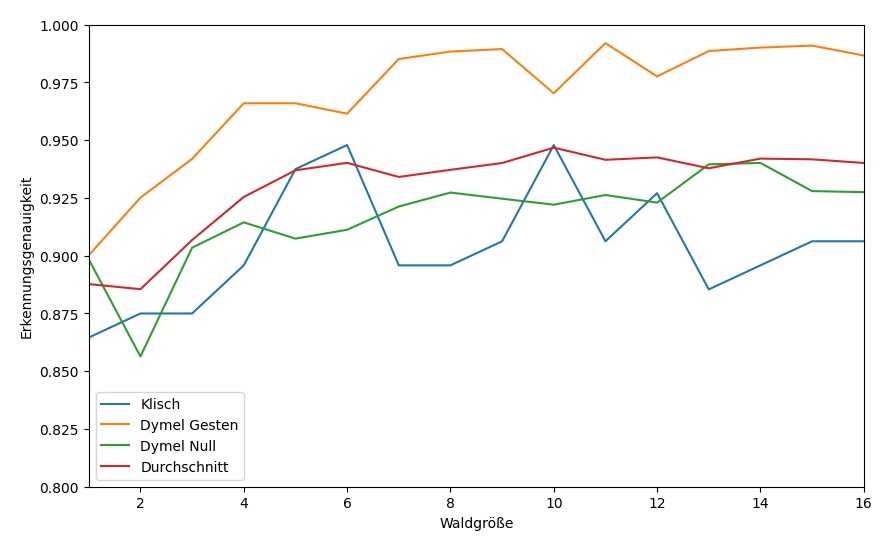
\includegraphics[width=\linewidth]{images/cocd_float_acc_per_size.png}
    \caption{Die beste summierte Erkennungsgenauigkeit pro Waldgröße der Schwerpunktverteilung mit Gleitkommazahlen.}
    \label{fig:cocd_float_per_forest_size}
\end{figure}
Die Featuremenge Schwerpunktverteilung mit Gleitkommazahlen folgt der Definition aus Sektion \ref{sec:schwerpunktverteilung} und beinhaltet insgesamt 10 Einträge, wobei jeweils 2 Einträge die X und Y
Koordinate des Schwerpunktes darstellen in insgesamt 5 Zeitfenstern.
\newline
\newline
Die beste Konfiguration wurde mit der Ensemble-Methode Boosting erzielt (siehe Tabelle \ref{tab:schwerpunktverteilung_float}). Mit einer Erkennungsgenauigkeit von 94,8\% auf der Testmenge von Klisch
ist dieser Ansatz nur 5,2\% schlechter als das neuronale Netz von Giese \cite{gieseThesis}. Es ist anzumerken, dass mit einer kleineren Trainingsmenge ohne die Gestentrainingsmenge und Nullgestentrainingsmenge eine Lösung
gefunden wurde, die 97,9\% erzielte und damit nur 2,1\% schlechter ist. Außerdem werden 97\% der Gestentestmenge und 92,2\% der Nullgestentestmenge korrekt klassifiziert.
\newline
\newline
Im Vergleich zu der Helligkeitsverteilung und Motion History ist die Erkennungsgenauigkeit dieses Ansatzes signifikant besser, sogar wenn nur 6656 Byte Programmspeicher verwendet werden. Wird die beste Konfiguration mit
der \textit{Unter 14 kB} verglichen, nimmt die Gesamterkennungsganuigkeit nur um 4,17\% ab bei der Reduktion der Programmgröße von 92\%. Dies verspricht, dass mit zunehmender Waldgröße der die Erkennungsgenauigkeit steigt.
Abbildung \ref{fig:cocd_float_per_forest_size} zeigt, dass dies zwar der Fall ist, aber schon ab einer Waldgröße von 6 ist die Durchschnittliche Erkennungsgenauigkeit keinen signifikanten Zuwachs mehr verzeichnet.
Dementsprechend ist der Unterschied der Gesamterkennungsgenauigkeit der besten Konfiguraiton und \textit{Unter 60 kB} mit 0,7\% nicht groß, wodurch sich dieses Feature gut für kleine eingebettete Systeme mit
wenig Programmspeicher eignet.
\subsection{Schwerpunktverteilung mit Ganzzahlen}
\begin{table}[h!]
    \hspace{-0.5cm}
    \begin{tabular}{ | l | c | c | c |}
        \hline
        Konfiguration & Beste & Unter 44 kB \& 28 kB & Unter 14 kB \\\hline
        Ensemble-Methode & ExtraTrees & Random Forest & Random Forest \\\hline
        Maximalhöhe & 21 & 13 & 12 \\\hline
        Waldgröße & 11 & 7 & 3 \\\hline
        Blattgröße (min\_samples\_leaf) & 2 & 4 & 1 \\\hline
        Programmgröße in Bytes & 76200 & 21532 & 11012 \\\hline
        Genauigkeit Testmenge von Klisch & 95,8\% & 91,7\% & 86,5\% \\\hline
        Genauigkeit Gestentestmenge & 98,8\% & 97,1\% & 95,5\% \\\hline
        Genauigkeit Nullgestentestmenge & 95,6\% & 94,5\% & 88,9\% \\\hline
    \end{tabular}
    \caption{Die besten Konfigurationen der Schwerpunktverteilung mit Ganzzahlen.}
    \label{tab:schwerpunktverteilung_int}
\end{table}
\begin{figure}[h!]
    \centering
    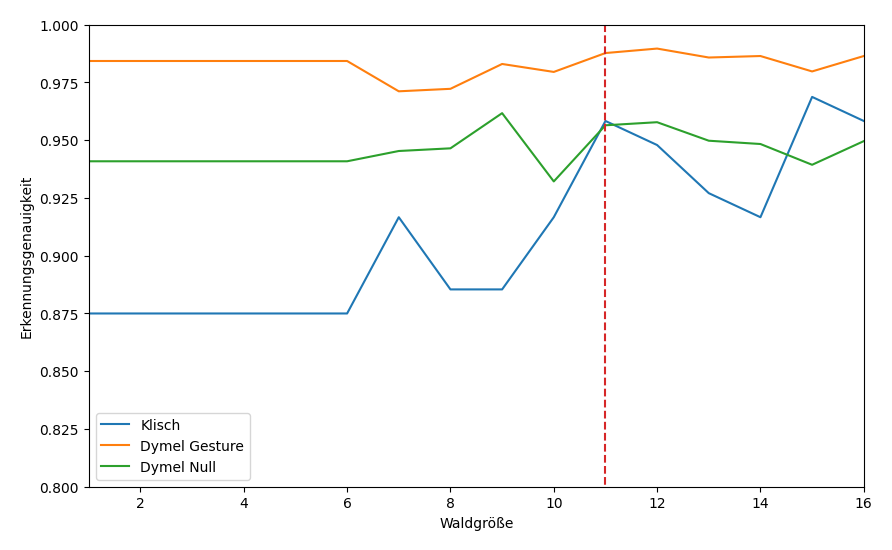
\includegraphics[width=\linewidth]{images/cocd_int_acc_per_size.png}
    \caption{Die besten Konfigurationen pro Waldgröße der Schwerpunktverteilung mit Ganzzahlen.}
    \label{fig:cocd_int_per_forest_size}
\end{figure}
Die Featuremenge Schwerpunktverteilung mit Ganzzahlen folgt der Definition aus Kapitel \ref{sec:schwerpunktverteilung} und beinhaltet insgesamt 10 Einträge. Jeweils 2 Einträge bilden die X und Y
Koordinate des Schwerpunktes. Damit spiegeln 10 Einträge insgesamt 5 Zeitfenster wieder.
\newline
\newline
Aus der Tabelle \ref{tab:schwerpunktverteilung_int} sind die besten Konfigurationen jeder Kategorie zu entnehmen. Die beste Konfiguration wurde mit der Ensemble-Methode ExtraTrees gefunden.
Mit einer Klassifizierungsgenauigkeit von 95,8\% auf der Testmenge von Klisch ist dieser Ansatz nur 3,2\% schlechter als das neuronale Netz von Giese \cite{gieseThesis}. Es wurde aber auch eine Konfiguration
gefunden, die 96,9\% der Testmenge von Klisch korrekt klassifiziert und damit nur 2,1\% schlechter ist. Diese maximiert aber in keiner Kategorie die Gesamtklassifizierungsgenauigkeit.
Außerdem werden 98,8\% der Gestentestmenge und 95,6\% der Nullgestentestmenge korrekt klassifiziert. Es wurde kein Entscheidungswald gefunden, der weniger als 44 kB Programmspeicher benötigt und besser ist als die
Konfiguration in der Kategorie \textit{Unter 28 kB}.
\newline
\newline
Der Ansatz mit Ganzzahlen erzielte eine 2,1\% höhere Gesamtklassifizierungsgenauigkeit als der Ansatz mit Gleitkommazahlen. Der 16-Bit Integer Datentyp erlaubt der Schwerpunktverteilung mit Ganzzahlen unter jeder
Restriktion größere Entscheidungswälder zu bilden, als die Schwerpunktverteilung mit Gleitkommazahlen. Abbildung \ref{fig:cocd_int_per_forest_size} zeigt einen Zuwachs der durchschnittlichen Klassifizierungsgenauigkeit
mit zunehmender Waldgröße. Es ist auszugehen, dass eine noch bessere Konfiguration gefunden werden könnte, wenn der Suchraum auf eine größere Waldgröße erweitert wird. Ähnlich wie die Schwerpunktverteilung mit
Gleitkommazahlen ist der Zuwachs der durchschnittlichen Klassifizierungsgenauigkeit ab einer Waldgröße von 7 Bäumen gering. Somit kann bereits bei einer geringen Programmgröße eine hohe Klassifizierungsgenauigkeit
erzielt werden. Damit eignet sich die Schwerpunktverteilung mit Ganzzahlen ebenfalls für kleine eingebettete Systeme.

\subsection{Kombinierte Schwerpunktverteilung}
\begin{table}[h!]
    \centering
    \begin{tabular}{ | l | c | c | c | c |}
        \hline
        Konfiguration & Beste & Unter 44 kB & Unter 28 kB \\\hline
        Schwerpunktverteilung Gleitkommazahl & Beste & Unter 14 kB & Unter 14 kB \\\hline
        Schwerpunktverteilung Ganzzahlen & Beste &  Unter 28 kB & Unter 14 kB \\\hline
        Programmgröße in Bytes & - & 33276 & 20252 \\\hline
        Genauigkeit Testmenge von Klisch & 94,8\% & 87,5\% & 87,5\% \\\hline
        Genauigkeit Gestentestmenge & 99,0\% & 97,7\% & 96,9\% \\\hline
        Genauigkeit Nullgestentestmenge & 95,8\% & 92,9\% & 92,5\% \\\hline
    \end{tabular}
    \caption{Die besten Konfigurationen der kombinierten Schwerpunktverteilung.}
    \label{tab:schwerpunktverteilung_int_and_float}
\end{table}
Die kombinierte Schwerpunktverteilung vereint die Schwerpunktverteilung mit Ganzzahlen und Gleitkommazahlen. Das erscheint sinnvoll, da der Ansatz mit Ganzzahlen invariant zu einem Offset in der
Helligkeit ist und der Ansatz mit Gleitkommazahlen invariant zur Skalierung der Helligkeit.
\newline
\newline
Es wird davon ausgegangen, dass der jeweilige Klassifizierer entweder ein Ergebnis mit einer deutlichen Mehrheit zurückgibt oder ein Ergebnis mit einer knappen Mehrheit. Für jedes Lichtverhältniss, hat mindestens ein
Klassifizierer eine deutliche Mehrheit. Damit erzielt die Kombination eine Mehrheit bei der korrekten Klasse. Die besten Konfigurationen der beiden Ansätze werden mit einem Wahlklassifizierer vereint.
Das heißt, die Wahrscheinlichkeitsverteilungen der Wahlklassifizierer der jeweiligen Ansätze werden zu gleichen Anteilen addiert.
\newline
\newline
Die Kombination der besten Konfigurationen beider Ansätze erzielt eine Klassifizierungsgenauigkeit von 94,8\% auf der Testmenge von Klisch. Dies entspricht der Klassifizierungsgenauigkeit der Schwerpunktverteilung mit
Gleitkommazahlen. 99\% der Gestentestmenge wird korrekt klassifiziert. Das ist besser als beide Ansätze. Die Nullgestestmenge wurde zu 95,8\% korrekt klassifiziert. Dies entspricht der Klassifizierungsgenauigkeit der
Schwerpunktverteilung mit Ganzzahlen. Bei der Kategorie \textit{Unter 44 kB} und \textit{Unter 28 kB} wurde der kombinierte Klassifizierer nie schlechter als der schlechteste Ansatz auf dem die kombinierte
Schwerpunktverteilung basiert.
\newline
\newline
Der Nachteil dieses Ansatzes ist, dass sowohl die Feature-Menge mit Gleitkommazahlen, als auch für Ganzzahlen benötigt wird. Zum einen müssen immer beide Features berechnet werden und zum anderen kann jeder Klassifizierer
nur halb so viel Speicher nutzen. Dadurch ist die Klassifizierungsgenauigkeit jedes Klassifizierers potenziell geringer, als wenn es den vollständigen Speicher zur Verfügung hätte. Bei der Schwerpunktverteilungen ist aber
bereits ab einer geringen Waldgröße kein signifikanter Zuwachs der Klassifizierungsgenauigkeit zu verzeichnen. Deswegen eignet sich die Schwerpunktverteilung besonders gut. Der Vorteil ist, dass der kombinierte
Klassifizierer potenziell robuster ist gegenüber unterschiedliche Lichtverhältnisse.


\subsection{Robustheit gegenüber Lichtverhältnisse}
TODO: For each best configuration per featureset add a line in the plot for scaling and offset invariance.


\section{Ausführungszeit}
\label{sec:eval_speed}
Die Ausführungszeit der Feature-Extrahierung und Klassifizierung ist ausschlaggebend für die mögliche FPS. Diese ermöglicht die Wahrnehmung von schnellen Handgesten. Ist die FPS bereits ausreichend
können leistungschwächere Module verwendet werden, wodurch die Batterielaufzeit verlängert wird oder die Kosten reduziert werden.
\newline
\newline
In dieser Arbeit wird das Arduino Board ATmega328P genutzt. Dieses Board verfügt über eine 8-Bit APU, 2 kB RAM, 32 kB Flash-Speicher und operiert unter 16 MHz \cite{atmega328p}.
Es verfügt nicht über ein Modul zur Verarbeitung von Gleitkommazahlen. Aus diesem Grund sind Operationen mit Gleitkommazahlen besonders teuer und zu vermeiden.
\newline
\newline
Es wird ausschließlich die \textit{Worst-Case-Execution-Time} (WCET) betrachtet. Ausschlaggebend dafür ist der \textit{Worst-Case-Execution-Path} (WCEP) im Kontrollflussgraph \cite{wcc_intro}. Der WCEP
setzt sich zusammen aus dem Vorgang das aktuelle Bild auszulesen, der Extrahierung der Features und der Ausführung des Klassifizierers.
\newline
\newline
Die Auswertung bezieht sich auf die Instruktionen des Programms, die bei der Übersetzung der Firmware durch den \textit{AVR GCC} mit der Optimierungsstufe \texttt{Os} entstehen. Aus dem Handbuch des
ATmega328P \cite{atmega328p} können für jede Instruktion die maximale Anzahl der Zyklen entnommen werden, die im schlimmsten Fall benötigt werden. Die Gesamtausführungszeit berechnet sich aus der Anzahl der Zyklen
multipliziert mit der Zeit pro Zyklus, d. h. bei 16 MHz bedarf ein Zyklus 0,0625 $\mu s$.

\subsection{Feature-Extrahierung}
Die Feature-Extrahierung implementiert die Berechnung der fünf Zeitfenster für die Schwerpunktverteilung. Einerseits muss aus jedem Bild der Schwerpunkt berechnet werden und andererseits müssen die Schwerpunkte
auf fünf Schwerpunkte zusammengefasst werden, die die fünf Zeitfenster repräsentieren.
\newline
\newline
Jedes Mal wenn ein Bild aufgenommen wird, wird der Schwerpunkt dieses Bildes berechnet und gespeichert. Dies reduziert einerseits die WCET, da im WCEP weniger Schwerpunkte berechnet werden müssen, und andererseits
wird weniger Pufferspeicher benötigt pro Bild. Für Gleitkommazahlen reduziert sich der Verbrauch pro Bild von 18 Byte auf 8 Byte und für Ganzzahlen auf 4 Byte. Der kombinierte Ansatz muss beide Schwerpunkte speichern.
Die jeweiligen Schwerpunktkoordinaten berechnen sich mit der in Kapitel \ref{sec:schwerpunktverteilung} beschriebenen Formel. Dabei muss die Summe der Pixel einmalig pro Bild berechnet werden und jeweils die
berechnete X und Y Koordinate im Puffer für den derzeitige Schwerpunkt gespeichert werden. Listing \ref{lst:cocdAlgoCOCDPerPicture} zeigt, wie dies auf dem ATmega328P implementiert ist. Insgesamt werden bei der
Schwerpunktverteilung mit Gleitkommazahlen 201 Zyklen für die einzelnen Instruktionen benötigt (12,5625 $\mu s$). Zusätzlich wird \textit{\_\_floatsisf} sechs mal aufgerufen, \textit{\_\_lesf2} und \textit{\_\_divsf3}
jeweils zwi mal aufgerufen. Die WCET zur Schwerpunktberechnung eines Bildes beläuft sich damit auf 116,5625 $\mu s$. Davon werden 104 $\mu s$ für Gleitkommaoperationen aufgewendet. Der Ansatz mit Ganzzahlen benötigt
keine Gleitkommaoperationen und 57 Zyklen weniger, da die summe der Pixel nicht berechnet werden muss, d. h. es werden für die WCET nur 8,875 $\mu s$ benötigt. Für den kombinierten Ansatz werden zusätzlich vier
Speicherinstruktionen benötigt, die einen Overhead von 0,25 $\mu s$ erzeugen, d. h. es werden für die WCET 116,8125 $\mu s$ benötigt.
\begin{lstlisting}[label=lst:cocdAlgoCOCDPerPicture,caption={Implementierung um den Schwerpunkt für ein Bild zu berechnen.}]
short helligkeits_summe = 0;
for (char i = 0; i < 9; ++i)
    helligkeits_summe += bild_puffer[i];
schwerpunkt_puffer_x[anzahl_bilder_im_puffer] = (float)(bild_puffer[0] + bild_puffer[3] + bild_puffer[6] - bild_puffer[2] - bild_puffer[5] - bild_puffer[8]) / ((float)helligkeits_summe);
schwerpunkt_puffer_y[anzahl_bilder_im_puffer] = (float)(bild_puffer[0] + bild_puffer[1] + bild_puffer[2] - bild_puffer[6] - bild_puffer[7] - bild_puffer[8]) / ((float)helligkeits_summe);
\end{lstlisting}
Wenn ein Handgestenkandidat detektiert wurde, wird für jedes Zeitfenster der Durchschnitt der darin enthaltenden Schwerpunkte berechnet. Die daraus berechneten Schwerpunkte werden als Schwerpunktverteilung bezeichnet.
Listing \ref{lst:cocdAlgo} zeigt den Algorithmus, um die Schwerpunktverteilung aus den Schwerpunkten im Puffer zu berechnen. Zunächst wird bei der Initialisierungsphase das \texttt{zusammenfass\_muster} berechnet
(Kap \ref{sec:schwerpunktverteilung}). Dafür werden im schlimmsten Fall 123 Zyklen für die einzelnen Instruktionen benötigt (7,6875 $\mu s$) und 20 $\mu s$ für die Ganzzahldividierung \textit{\_\_divmodhi4}. Insgesamt
27,6875 $\mu s$. Dieser Teil wird genau 1 mal für alle Richtungen und Schwerpunktverteilungen durchgeführt. Die innere Schleife wird im schlimmsten Fall für die Gesamtgröße des Schwerpunktpuffers durchlaufen.
Jeder Durchlauf benötigt im schlimmsten Fall 27 Zyklen für die einzelnen Instruktionen (1,6875 $\mu s$) und führt \textit{\_\_addsf3} einmal aus. Der WCET für einen Durchlauf beläuft sich damit auf 13,6875 $\mu s$.
Der Ansatz mit Ganzzahlen benötigt im schlimmsten Fall 17 Zyklen (1,125 $\mu s$). Bei einer Gesamtpuffergröße von 125 wird für den Teil der inneren Schleife für die Schwerpunktverteilung mit Gleitkommazahlen
1710,9375 $\mu s$ benötigt, für die Schwerpunktverteilung mit Ganzzahlen 140,625 $\mu s$ und für den kombinierten Ansatz 1851,5625 $\mu s$. Die äußere Schleife benötigt im schlimmsten Fall 57 Zyklen für die einzelnen
Instruktionen (3,5625 $\mu s$) und ruft im Ansatz mit Gleitkommazahlen fünf mal \textit{\_\_floatsisf} und \textit{\_\_divsf3} auf und im Ansatz mit Ganzzahlen fünf mal \textit{\_\_divmodhi4}. Damit beläuft sich der WCET
bei fünf Durchläufen der äußeren Schleife für den Ansatz mit Gleitkommazahlen auf 217,8125 $\mu s$, für den Ansatz mit Ganzzahlen auf 117,8125 $\mu s$ und für den kombinierten Ansatz 335,625 $\mu s$.
\begin{lstlisting}[label=lst:cocdAlgo,caption={Algorithmus um die Schwerpunktverteilung in horizontaler Richtung zu berechnen.}]
Initialisierung.
for (char i = 0; i < 5; ++i) { // Äußere Schleife
    features[i] = 0;
    for (char j = 0; j < zusammenfass_muster[i]; ++j) // Innere Schleife
        features[i] += *(schwerpunkt_puffer_x++);
    features[i] /= ((float)zusammenfass_muster[i]);
}
\end{lstlisting}
Der Schwerpunkt wird jeweils für die horizontale und vertikale Richtung berechnet. Der kombinierte Ansatz berechnet sowohl den Schwerpunkt für Gleitkommazahlen als auch für Ganzzahlen. Die WCET für die Feature-Extrahierung
der Schwerpunktverteilung mit Gleitkommazahlen beläuft sich auf 4001,75 $\mu s\ \approx\ $ 4 ms. Die WCET der Schwerpunktverteilung mit Ganzzahlen beläuft sich auf 553,4375 $\mu s\ \approx\ $ 0,6 ms. Die WCET der kombinierten
Schwerpunktverteilung beläuft sich auf 4518,875 $\mu s\ \approx\ $ 4,5 ms.

\subsection{Tree Evaluation}
\subsection{Ausführung eines Entscheidungswaldes}
Der WCEP eines Entscheidungswaldes setzt sich aus dem WCEP des Wahlklassifizierungsalgorithmus und dem WCEP jedes Entscheidungsbaumes zusammen, der im Wald enthalten ist.
\newline
\newline
Der in Listing \ref{lst:sklearnCCodeTreeVoting} gezeigte Code implementiert den Wahlvorgang. Die Komplexität ist abhängig von der Anzahl der Features $N$ und der Anzahl der Entscheidungsbäume $K$. In
dieser Analyse wird für die Anzahl der Features $N=5$ angenommen.
Jede Stimme eines Entscheidungsbaumes bedarf 18~Zyklen (1,125~$\mu s$), um die Funktion, die den Entscheidungsbaum ausführt, aufzurufen und das Ergebnis des ausgeführten Entscheidungsbaumes auf die Gesamtsumme zu addieren.
Die restlichen Instruktionen bedürfen 64 Zyklen (4~$\mu s$).
\newline
\newline
Die WCET eines Entscheidungswaldes beläuft sich damit auf 4~$\mu s$ + \#Entscheidungsbäume $\cdot$ (1,125~$\mu s$ + WCET der Entscheidungsbäume).
\section{Programmgröße}
\label{sec:eval_size}
Generell gilt, je größer und dichter der Entscheidungswald ist, desto höher ist die Erkennungsgenauigkeit. Aus diesem Grund sollte immer der vollständige Programmspeicher ausgenutzt werden. Allerdings nimmt der
Zuwachs an Erkennungsgenauigkeit mit jeder weiteren Teilung ab bei der Konstruktion eines Entscheidungsbaumes.
\newline
\newline
Scikit-Learn bietet viele Parameter, um die Teilung zu steuern. Dies mag die potentielle
Erkennungsgenauigkeit eines Baumes leicht verringern, kann dafür aber die Größe stark verringern. Dadurch jönnen tiefere Bäume verwendet werden oder mehr Bäume in einem Entscheidungswald, was potentiell
einen größeren Zuwachs der Erkennungsgenauigkeit verspricht.
\newline
\newline
Die Größe und Dichte eines Entscheidungswaldes haben einen direkten Einfluss auf die generierten Instruktionen. Je größer und dichter, desto mehr Instruktionen. Aus diesem Grund soll einerseits der
Zuwachs der Erkennungsgenauigkeit pro Vergleich maximiert werden und andererseits die Instruktionskosten pro Vergleich und Blattkosten minimiert werden.

\subsection{Maximierung des Zuwachses der Klassifizierungsgenauigkeit}
Scikit-Learn bietet viele Parameter an, um den Teilungsprozess bei der Konstruktion zu steuern. Einer dieser Parameter ist \texttt{min\_samples\_leaf}, d. h. die minimale Anzahl an Einträgen der Trainingsmenge
in einem Blatt. Dieser steuert die minimale Anzahl an Einträgen die in einem Kindknoten enthalten sein müssen, nachdem ein Knoten geteilt wurde. Standardmäßig ist der Wert 1. Dadurch entsteht ein sehr fein granularer
Entscheidungsbaum, der viele Blätter mit nur einem Eintrag hat. Das heißt, es wurden Teilungen durchgeführt, die nur zwei Einträge unterteilt haben. Der Zuwachs der Klassifizierungsgenauigkeit ist durch diese
Teilungen sehr gering. Eine Erhöhung in der Blattgröße verspricht, dass Entscheidungsbäume gefunden werden können, die zwar tiefer sind, aber dafür eine bessere Klassifizierungsgenauigkeit pro Vergleich erzielen.
Der Baum kann tiefer werden, da die Grenze des Programmspeichers noch nicht erreicht wurde.
\newline
\newline
Abbildung \ref{fig:msl} zeigt, wie sich der Parameter auf verschieden große Trainingsmengen auswirkt. Betrachtet wird eine Maximalhöhe von 16. Besonders bei großen Trainingsmengen (Abbildung \ref{subfig:msl_big})
kann die Programmgröße mit einer Blattgröße von 8 signifkant sinken, ohne die maximale Baumhöhe zu beeinflussen. Bei kleinen Trainingsmengen (Abbildung \ref{subfig:msl_small}) reduziert bereits bei kleinen Blattgrößen
sich die Programmgröße ebenfalls signifikant. Allerdings wird die maximale Baumhöhe beeinflusst. Besonders bei großen Trainingsmengen wirkt sich der Parameter stärker auf die Programmgröße aus.
Vermutlich, da die Anzahl der Blätter sich signifikant erhöht, je tiefer der Baum ist.
\subfigbox{
\subfigure[Trainingsmengengröße: 1023]{\label{subfig:msl_small}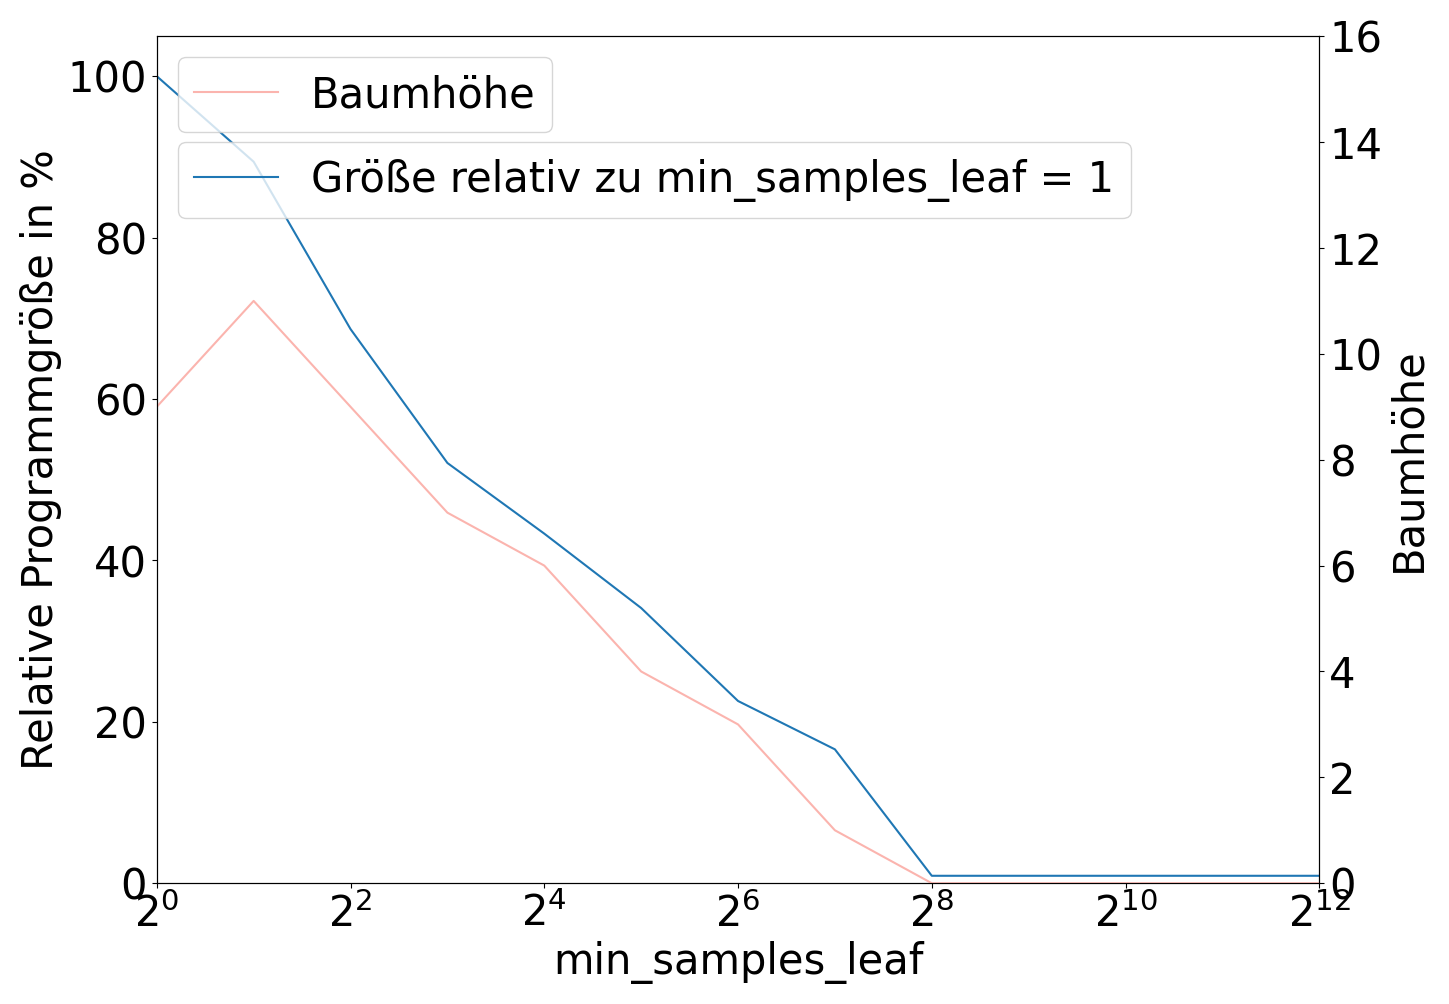
\includegraphics[width=0.48\linewidth]{images/min_samples_leaf_small.png}}\hfill%
\subfigure[Trainingsmengengröße: 7629]{\label{subfig:msl_big}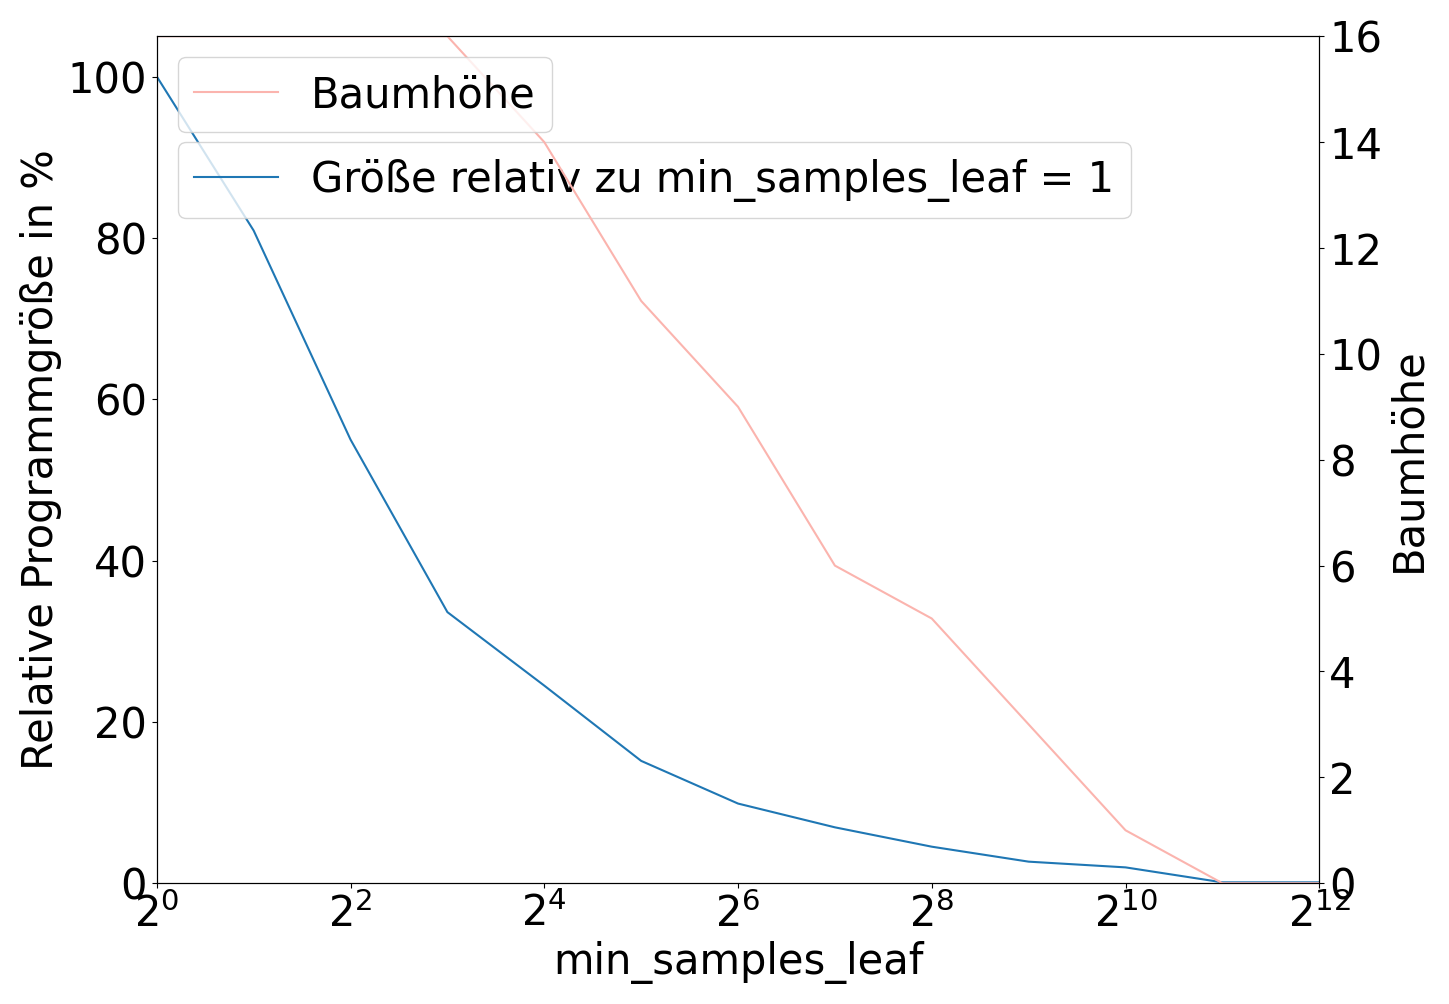
\includegraphics[width=0.48\linewidth]{images/min_samples_leaf_big.png}}%
}{Auswirkung der minimalen Blattgröße auf Programmgröße und Baumhöhe.}{fig:msl}
\newline
\newline
Es kann nicht argumentiert werden, dass ein Wert für die Blattgröße besser ist als ein Anderer, da die Klassifizierungsgenauigkeit auf der Trainingsmenge keine Aussage über die Klassifizierungsgenauigkeit auf
der Testmenge treffen kann. Eine hohe Klassifizierungsgenauigkeit auf Trainingsmenge muss nicht umbedingt eine hohe Klassifizierungsgenauigkeit auf der Testmenge implizieren. Allerdings können so vermeintlich
höhere Entscheidungsbäume ausgewählt werden, da diese weniger Programmspeicher benötigen im Vergleich zu gleich hohen Entscheidungsbäumen mit einer geringeren Blattgröße. Dieser Parameter vergrößert folglich
den Suchraum. Bei kleinen Trainingsmengen ist eine Blattgröße über 1 nur sinnvoll, wenn der größte Entscheidungsbaum, der generiert werden kann, nicht innerhalb der Restriktionen des Programmspeichers liegt.
\subsection{Minimierung der Instruktionen eines Vergleichs}
Ein Vergleich in einem Entscheidungsbaum wurde in Kapitel \ref{sec:cCodeTree} als Abzweigungsexpression mit einem Test definiert. Der Compiler erzeugt für den gleichen Programmcode verschieden viele Instruktionen
je nach Wahl des Datentyps.
\newline
\newline
Listing \ref{lst:assemblyVergleich} zeigt die Komplexität eines einzigen Vergleichs in Instruktionen eines Gleitkommazahlvergleichs. Zeile 1 bis 4 lädt die konstante Gleitkommazahl in 4 hintereinander liegende
8-Bit Register. Zeile 5 bis 7 lädt den Zeiger, der auf die Feature-Menge zeigt, und inkrementiert ihn um 36, um auf das 9. Feature zuzugreifen. In Zeile 8 bis 11 wird das Feature in die Register geladen. Zeile 12 bis 15 führen die
Vergleichsfunktion aus. Damit benötigt ein Vergleich insgesamt 15 Instruktionen.
\begin{lstlisting}[label=lst:assemblyVergleich,caption={Vergleich von Feature als Gleitkommazahl mit konstanter Gleitkommazahl.}]
01: ldi r18,lo8(33)
02: ldi r19,lo8(-92)
03: ldi r20,lo8(69)
04: ldi r21,lo8(60)
05: ldd r26,Y+5
06: ldd r27,Y+6
07: adiw r26,36
08: ld r22,X+
09: ld r23,X+
10: ld r24,X+
11: ld r25,X
12: sbiw r26,36+3
13: call __lesf2
14: cp __zero_reg__,r24
15: brge .+2
\end{lstlisting}
Zu vermeiden sind Zeile 5 bis 11, indem alle Features nur einmal in Register geladen werden. Dies ist allerdings nur möglich, wenn die Größe der Feature-Menge nicht 32~Byte übersteigt bei dem
ATmega328P. Zusätzlich müssten noch Bytes verfügbar sein, um die Konstanten zu laden. Die Feature-Menge der Schwerpunktverteilung beinhaltet 10 Einträge. Der Ansatz mit Gleitkommazahlen ist mit 40 Bytes zu groß.
Der Ansatz mit Ganzzahlen kann diese Optimierung mit 20~Byte ausnutzen. Der Compiler führt diese Optimierung bereits automatisch durch. Wenn die Feature-Menge zu groß ist, werden aus diesem Grund regelmäßig
Register verdrängt, wodurch zusätzlich Instruktionen entstehen. Die Anzahl der Instruktionen können reduziert werden, indem die Größe der Feature-Menge reduziert wird, sodass die Feature-Menge und eine
zusätzliche Konstante des gleichen Datentyps den Registerspeicher nicht übersteigen.
\newline
\newline
Der Datentyp \texttt{Float} ist sehr teuer für einen 8-Bit Prozessor, da immer 4~Register benötigt werden und gegebenenfalls zusätzliche Funktionen, die die fehlende Hardwareunterstüzung ergänzen.
Idealerweise sollte für die Feature-Menge und die Vergleiche ein 8-Bit Datentyp gewählt werden. Damit werden einerseits weniger Register benötigt, wodurch wiederrum die Feature-Menge größer sein kann,
und andererseits können hardwareunterstützte Vergleichsinstruktionen benutzt werden. Dies verringert die Anzahl der Instruktionen signifikant. Folglich vermindert ein kleinerer Datentyp die Anzahl der
Instruktionen signifikant. Listing \ref{lst:assemblyVergleich8Bit} zeigt einen Vergleich von einem 8-Bit Datentyp. Im Kontrast zum Vergleich mit Gleitkommazahlen, werden 66,6\% weniger Instruktionen
benötigt.
\begin{lstlisting}[label=lst:assemblyVergleich8Bit,caption={Vergleich von 8-Bit Feature mit konstanter 8-Bit Zahl.}]
01: adiw r26,4
02: ld r24,X
03: sbiw r26,4
04: cpi r24,lo8(124)
05: brge .L3
\end{lstlisting}
\subsection{Minimierung der Instruktionen einer Rückgabe}
Die Rückgabe der Klassifizierung in einem Entscheidungsbaum kann auf zwei Arten stattfinden. Einerseits kann lediglich die Klasse mit der höchsten Wahrscheinlichkeit zurückgegeben werden. Andererseits kann die
Wahrscheinlichkeitsverteilung zurückgegeben werden, sodass die nächste Ebene die Entscheidung trifft. In Kapitel \ref{sec:cCodeTree} wurde letzteres vorgestellt, da in der nächsten Ebene der Wahlklassifizierer
die Entscheidungsbäume im Ensemble mit Hilfe ihrer Wahrscheinlichkeitsverteilungen zusammenfasst.
\newline
\newline
Listing \ref{lst:assemblyBlattReturn} zeigt die Instruktionen die für die Zuweisung zu vier Klassen von 1.0, 0.0, 0.0 und 0.0 generiert werden. Für jede Klasse wird die Konstante Wahrscheinlichkeit in Register geladen
und anschließend in den Rückgabeparameter gespeichert. In diesem Fall muss nur für die erste Klasse eine Konstante geladen werden, da jede andere Klasse 0 ist. Das heißt, dass im schlimmsten Fall 33
Instruktionen benötigt werden, anstatt 21. Der Compiler führt hier bereits eine Optimierung aus, indem für jedes Ergebnis ein eigener \textit{Basic block} (Eine Datenstruktur die Instruktionen mit einer Annotation
zusammenfasst)erzeugt wird. Zusätzlich könnte kein C-Code generiert werden für eine Zuweisungen mit 0. Dies erfordert aber, dass der Rückgabeparameter mit 0 vorinitialisiert ist.
\newpage
\begin{lstlisting}[label=lst:assemblyBlattReturn,caption={Beispiel der Instruktionen einer Rückgabe der Wahrscheinlichkeitsverteilung eines Entscheidungsbaumes mit 4~Klassen.}]
01: ldi r24,0
02: ldi r25,0
03: ldi r26,lo8(-128)
04: ldi r27,lo8(63)
05: st Z,r24
06: std Z+1,r25
07: std Z+2,r26
08: std Z+3,r27
09: std Z+4,__zero_reg__
10: std Z+5,__zero_reg__
11: std Z+6,__zero_reg__
12: std Z+7,__zero_reg__
13: std Z+8,__zero_reg__
14: std Z+9,__zero_reg__
15: std Z+10,__zero_reg__
16: std Z+11,__zero_reg__
17: std Z+12,__zero_reg__
18: std Z+13,__zero_reg__
19: std Z+14,__zero_reg__
20: std Z+15,__zero_reg__
21: ret
\end{lstlisting}
Eine weitere Optimierung ist den Wahlklassifizierer diskret zu modellieren. Dabei wird für jede Rückgabe des Entscheidungsbaumes ein einstimmiges Ergebnis angenommen, d. h. es wird die Klasse mit der
höchsten Wahrscheinlichkeit in jedem Baum zurückgegeben und nicht mehr die Wahrscheinlichkeitsverteilung. Dadurch werden lediglich die erkannten Klassen
gezählt, anstatt die Wahrscheinlichkeitsverteilungen zu addieren. Listing \ref{lst:assemblyBlattReturnDiskret} zeigt, dass sich die Anzahl der Instruktionen für eine Rückgabe auf genau 2~Instruktionen
reduzieren. Zusätzlich kann der Compiler diese Rückgabe in Basic blocks extrahieren, wodurch lediglich eine Sprunginstruktion benötigt wird. Diese Optimierung ist bei dem diskreten Wahlklassifizierer noch
effektiver, da es genau $N$ verschiedene Rückgabewerte gibt, für $N$ mögliche Klassen. Im schlimmsten Fall reduzieren sich die Anzahl der Instruktionen pro Rückgabe um $\frac{100}{1 + 4N}$\%
und im besten Fall um $\frac{100}{1 + 8N}$\%.
\begin{lstlisting}[label=lst:assemblyBlattReturnDiskret,caption={Beispiel des Assemblycodes der Rückgabe eines diskreten Wahlklassifizierers.}]
01: ldi r24,lo8(1)
02: ret
\end{lstlisting}
Der Nachteil dieses Ansatzes ist, dass die Ergebnisse instabil werden können, wenn viele Rückgaben nur über eine knappe Mehrheit verfügen. Das ist insbesondere der Fall in Kombination mit einem hohen Wert
für die Blattgröße, da dieser die Anzahl der Blattknoten mit Einträgen aus verschiedenen Klassen potenziell erhöht. Diese Optimierung kann auf eine gefundene Lösung angewendet werden, die zu groß für den
Programmspeicher ist. Anschließend sollte die Klassifizierungsgenauigkeit revalidiert werden. Tests haben ergeben, dass die Klassifizierungsgenauigkeit geringfügig schwankt. Folglich kann sich die
Klassifizierungsgenauigkeit auf der Testmenge auch erhöhen.
\newline
\newline
Denkbar wäre ein hybrider Ansatz, der bei einem eindeutigen Ergebnis die Klasse zurück gibt und ansonsten die Wahrscheinlichkeitsverteilung. Die \glqq Eindeutigkeit\grqq\ kann über
einen Schwellenwert $\delta$ definiert sein. Ein Schwellenwert von $\delta=0$ würde an der Korrektheit nichts ändern, würde aber im schlimmsten Fall die Programmgröße nicht verringern.
Tests haben ergeben, dass es immer eindeutige Ergebnisse gibt, weswegen diese Optimierung immer angewendet werden sollte.
